\chapter{Military \& Covert Communications}
\label{ch:military-covert}

\begin{nontechnical}
\textbf{Military communications are like having a secret conversation in a hostile crowd}---you need to avoid being heard by enemies, resist jamming, and stay undetected.

\textbf{Key concepts in simple terms:}
\begin{itemize}
\item \textbf{Spread Spectrum} = Whispering your message across a huge room so each piece sounds like background noise
\item \textbf{Frequency Hopping} = Changing radio channels thousands of times per second following a secret pattern
\item \textbf{Phased Arrays} = Computer-controlled antenna spotlights that instantly point anywhere
\item \textbf{Low Probability of Detection (LPD)} = Your signal is literally weaker than background noise
\end{itemize}

\textbf{Real example:} GPS M-code is 20 times weaker than noise, yet military receivers lock on instantly. Enemy receivers? Just static.

\textbf{Why it matters:} These techniques enable communications that survive 10,000× stronger jamming signals and remain invisible to adversaries.
\end{nontechnical}

\section{Overview}

Military communications systems prioritize \textbf{anti-jamming (AJ)}, \textbf{low probability of intercept (LPI)}, \textbf{low probability of detection (LPD)}, and \textbf{secure transmission (TRANSEC)} over commercial metrics like spectral efficiency.

\begin{keyconcept}
Processing gain from spread spectrum enables military links to operate 20--40~dB below the noise floor while overcoming jammers that are thousands of times stronger than the desired signal.
\end{keyconcept}

This chapter covers advanced techniques used in:
\begin{itemize}
\item GPS M-code (military GPS with anti-jam)
\item SATCOM FHSS (frequency hopping satellites)
\item Phased-array radar (AESA systems)
\item Link 16 (tactical data network)
\item Covert communications (LPD/LPI techniques)
\end{itemize}

\section{Mathematical Description}

\subsection{The LPI/LPD/AJ Triad}

Military communications are governed by three interrelated requirements:

\textbf{1. Low Probability of Intercept (LPI):} Enemy can detect transmission but cannot decode it.

\textbf{2. Low Probability of Detection (LPD):} Enemy cannot detect that transmission is occurring.

\textbf{3. Anti-Jamming (AJ):} Maintain link under deliberate enemy interference.

\subsection{Processing Gain}

The fundamental parameter enabling all three capabilities is \textbf{processing gain}:
\begin{equation}
G = \frac{BW_{\text{spread}}}{BW_{\text{info}}} = \frac{R_{\text{chip}}}{R_{\text{bit}}}
\end{equation}
where:
\begin{itemize}
\item $G$ = processing gain (ratio)
\item $BW_{\text{spread}}$ = spread bandwidth (Hz)
\item $BW_{\text{info}}$ = information bandwidth (Hz)
\item $R_{\text{chip}}$ = chip rate (chips/second)
\item $R_{\text{bit}}$ = bit rate (bits/second)
\end{itemize}

In decibels:
\begin{equation}
G_{\text{dB}} = 10 \log_{10}(G)
\end{equation}

\textbf{Power Spectral Density (PSD)} after spreading:
\begin{equation}
\text{PSD} = \frac{P_{\text{TX}}}{BW_{\text{spread}}}
\end{equation}
where:
\begin{itemize}
\item $P_{\text{TX}}$ = transmit power (W)
\item PSD = power per unit bandwidth (W/Hz)
\end{itemize}

\begin{calloutbox}{LPD Threshold}
For LPD, the signal PSD must be below the thermal noise floor. With processing gain $G > 30$~dB (factor of 1000), the spread signal becomes indistinguishable from background noise to wideband receivers.
\end{calloutbox}

\subsection{Jamming Margin}

The ability to overcome jamming is quantified by the \textbf{jamming margin}:
\begin{equation}
M_{\text{jam}} = G_{\text{dB}} - \frac{J}{S} - \left(\frac{E_b}{N_0}\right)_{\text{req}} - L
\end{equation}
where:
\begin{itemize}
\item $M_{\text{jam}}$ = jamming margin (dB), positive = link survives
\item $J/S$ = jammer-to-signal ratio at receiver (dB)
\item $(E_b/N_0)_{\text{req}}$ = required bit energy to noise ratio (dB)
\item $L$ = implementation losses (dB)
\end{itemize}

\begin{warningbox}
A positive jamming margin is essential for link survival. Military systems typically design for $M_{\text{jam}} \geq 10$~dB to account for fading and worst-case scenarios.
\end{warningbox}

\section{SATCOM Frequency Hopping (FHSS)}

Military satellite communications use Frequency Hopping Spread Spectrum (FHSS) for transmission security (TRANSEC) and anti-jamming.

\subsection{MILSTAR System Parameters}

\textbf{MILSTAR (Military Strategic and Tactical Relay)} specifications:
\begin{itemize}
\item Frequency: X-band uplink (7--8~GHz), Ka-band downlink (20--21~GHz)
\item Hop rate: 100--1000+ hops/second
\item Hop set: 1000+ frequencies across 1~GHz bandwidth
\item Dwell time: $<1$~ms per hop
\item Modulation: BPSK, QPSK, 8-PSK (adaptive)
\item Data rate: 75~bps to 1.544~Mbps
\item Constellation: 5 GEO satellites (global coverage)
\end{itemize}

\subsection{FHSS Processing Gain}

For frequency hopping, the processing gain is:
\begin{equation}
G_{\text{FH}} = N_{\text{hop}}
\end{equation}
where:
\begin{itemize}
\item $N_{\text{hop}}$ = number of frequencies in hop set
\end{itemize}

In decibels:
\begin{equation}
G_{\text{FH,dB}} = 10 \log_{10}(N_{\text{hop}})
\end{equation}

For MILSTAR with $N_{\text{hop}} = 1000$:
\begin{equation}
G_{\text{FH,dB}} = 10 \log_{10}(1000) = 30 \text{ dB}
\end{equation}

\subsection{LPI/LPD Analysis}

The power spectral density after frequency spreading:
\begin{equation}
\text{PSD} = \frac{P_{\text{TX}}}{BW_{\text{hop set}}}
\end{equation}

For MILSTAR ($P_{\text{TX}} = 100$~W, $BW_{\text{hop set}} = 1$~GHz):
\begin{equation}
\text{PSD} = \frac{100 \text{ W}}{10^9 \text{ Hz}} = 10^{-7} \text{ W/Hz} = -70 \text{ dBm/Hz}
\end{equation}

Thermal noise floor at 1~MHz bandwidth:
\begin{equation}
N = -174 \text{ dBm/Hz} + 10 \log_{10}(10^6) = -114 \text{ dBm/MHz}
\end{equation}

\begin{keyconcept}
The signal PSD ($-70$~dBm/MHz) is below the noise floor ($-114$~dBm/MHz when integrated over 1~MHz). This makes the transmission undetectable to wideband receivers without knowledge of the hopping pattern.
\end{keyconcept}

\subsection{Frequency Hopping Pattern Visualization}

\begin{center}
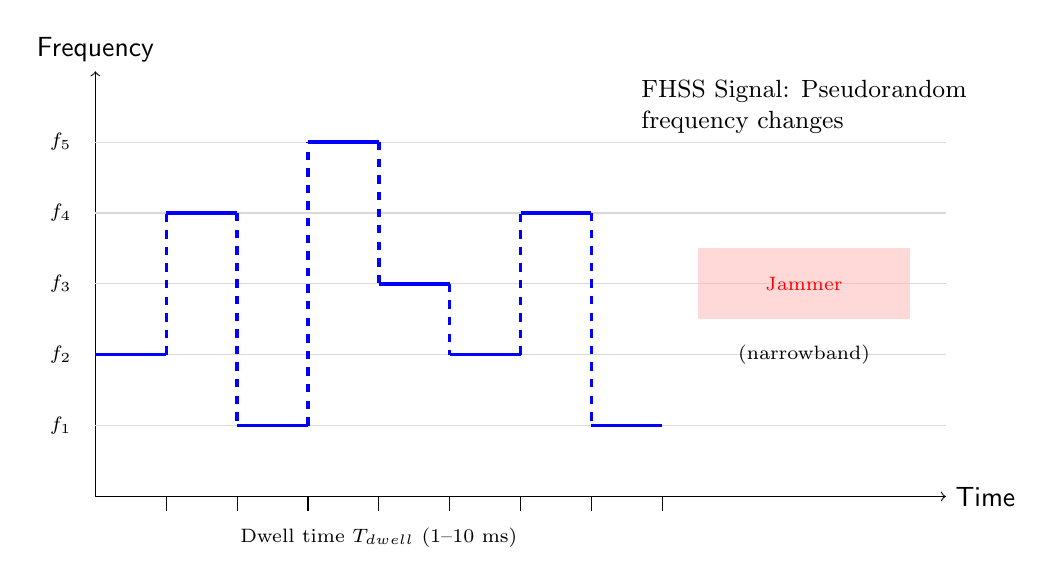
\begin{tikzpicture}[scale=0.9]
% Axes
\draw[->] (0,0) -- (12,0) node[right] {\sffamily Time};
\draw[->] (0,0) -- (0,6) node[above] {\sffamily Frequency};

% Frequency levels
\foreach \y in {1,2,3,4,5} {
  \draw[thin,gray!30] (0,\y) -- (12,\y);
  \node[left,font=\scriptsize] at (-0.2,\y) {$f_{\y}$};
}

% Hopping pattern (example sequence)
\draw[very thick,blue] (0,2) -- (1,2);
\draw[very thick,blue,dashed] (1,2) -- (1,4);
\draw[very thick,blue] (1,4) -- (2,4);
\draw[very thick,blue,dashed] (2,4) -- (2,1);
\draw[very thick,blue] (2,1) -- (3,1);
\draw[very thick,blue,dashed] (3,1) -- (3,5);
\draw[very thick,blue] (3,5) -- (4,5);
\draw[very thick,blue,dashed] (4,5) -- (4,3);
\draw[very thick,blue] (4,3) -- (5,3);
\draw[very thick,blue,dashed] (5,3) -- (5,2);
\draw[very thick,blue] (5,2) -- (6,2);
\draw[very thick,blue,dashed] (6,2) -- (6,4);
\draw[very thick,blue] (6,4) -- (7,4);
\draw[very thick,blue,dashed] (7,4) -- (7,1);
\draw[very thick,blue] (7,1) -- (8,1);

% Time slots
\foreach \x in {1,2,3,4,5,6,7,8} {
  \draw[thin] (\x,0) -- (\x,-0.2);
}
\node[below,font=\scriptsize] at (4,-0.3) {Dwell time $T_{\text{dwell}}$ (1--10 ms)};

% Jammer illustration
\fill[red!30,opacity=0.5] (8.5,2.5) rectangle (11.5,3.5);
\node[font=\scriptsize,red] at (10,3) {Jammer};
\node[font=\scriptsize] at (10,2) {(narrowband)};

% Legend
\node[font=\small,align=left] at (10,5.5) {FHSS Signal: Pseudorandom\\frequency changes};

\end{tikzpicture}
\end{center}

\textbf{Cryptographic synchronization:}
\begin{itemize}
\item Hopping pattern generated by NSA-approved algorithm
\item Synchronized using GPS time + Key Encryption Key (KEK)
\item Pattern period: days to weeks (appears never-repeating)
\end{itemize}

\subsection{FHSS Anti-Jam Performance}

\textbf{Scenario:} Tactical UHF link under jamming.

\textbf{Given parameters:}
\begin{itemize}
\item Processing gain: $G = 30$~dB (1000 hop set)
\item Jammer-to-signal ratio: $J/S = 40$~dB (jammer 10,000$\times$ stronger)
\item Required $E_b/N_0$: 10~dB (BPSK, BER $= 10^{-5}$)
\item Implementation losses: $L = 3$~dB
\end{itemize}

\textbf{Initial jamming margin:}
\begin{equation}
M_{\text{jam}} = 30 - 40 - 10 - 3 = -23 \text{ dB} \quad \text{(LINK FAILS)}
\end{equation}

\textbf{Countermeasure 1 -- Directional antenna:}
\begin{itemize}
\item Gain toward satellite: $+20$~dB
\item Null toward jammer: $-20$~dB
\item Effective $J/S = 40 - 20 = 20$~dB
\end{itemize}
\begin{equation}
M_{\text{jam}} = 30 - 20 - 10 - 3 = -3 \text{ dB} \quad \text{(MARGINAL)}
\end{equation}

\textbf{Countermeasure 2 -- Forward error correction:}
\begin{itemize}
\item Turbo/LDPC code rate-1/3: $+5$~dB coding gain
\end{itemize}
\begin{equation}
M_{\text{jam}} = -3 + 5 = +2 \text{ dB} \quad \text{(LINK SURVIVES)}
\end{equation}

\begin{calloutbox}{Layered Defense}
Military systems combine multiple anti-jam techniques: spread spectrum processing gain, directional antennas with nulling, forward error correction, and burst transmission. Each layer adds 3--20~dB of protection.
\end{calloutbox}

\subsection{Follower Jamming Resistance}

\textbf{Threat:} Smart jammer detects hop and jams that frequency.

Timing analysis for follower jammer defeat:
\begin{equation}
T_{\text{effective jam}} = T_{\text{dwell}} - (T_{\text{detect}} + T_{\text{switch}})
\end{equation}
where:
\begin{itemize}
\item $T_{\text{dwell}}$ = dwell time per frequency (ms)
\item $T_{\text{detect}}$ = jammer detection time ($\mu$s)
\item $T_{\text{switch}}$ = jammer frequency switching time ($\mu$s)
\end{itemize}

\textbf{Example -- MILSTAR defense:}
\begin{itemize}
\item Dwell time: $T_{\text{dwell}} = 1$~ms
\item Jammer detection: $T_{\text{detect}} = 100~\mu$s
\item Jammer switching: $T_{\text{switch}} = 50~\mu$s
\item Total jammer delay: $150~\mu$s
\end{itemize}
\begin{equation}
T_{\text{effective jam}} = 1000~\mu\text{s} - 150~\mu\text{s} = 850~\mu\text{s} \quad (85\% \text{ of hop})
\end{equation}

\textbf{Countermeasure -- Fast hopping:}
\begin{itemize}
\item Reduce dwell time: $T_{\text{dwell}} = 100~\mu$s (10$\times$ faster)
\end{itemize}
\begin{equation}
T_{\text{effective jam}} = 100~\mu\text{s} - 150~\mu\text{s} < 0 \quad \text{(jammer too slow!)}
\end{equation}

Modern military systems use $T_{\text{dwell}} = 10$--$100~\mu$s to defeat follower jammers.

\section{GPS M-Code (Military GPS)}

GPS Modernization provides jam-resistant, encrypted positioning for military users through M-code.

\subsection{Signal Structure}

\textbf{GPS L1 M-Code parameters:}
\begin{itemize}
\item Carrier frequency: $f_c = 1575.42$~MHz (L1 band)
\item Chip rate: $R_c = 5.115$~Mcps (5$\times$ faster than C/A code)
\item Code length: Classified (estimated $\sim 10^{13}$ chips, never repeats)
\item Modulation: BOC(10,5) -- Binary Offset Carrier
\item Processing gain: $\sim 50$~dB (vs. 43~dB for C/A)
\item Power: 6.5~dB stronger than C/A code
\item Security: Encrypted, NSA-authenticated
\end{itemize}

\textbf{GPS L2 M-Code:}
\begin{itemize}
\item Carrier frequency: $f_c = 1227.60$~MHz (L2 band)
\item Same structure as L1 M-code
\item Dual-frequency enables ionospheric correction
\end{itemize}

\subsection{BOC Modulation}

Binary Offset Carrier (BOC) modulates the chip sequence with a square wave subcarrier. For BOC($m$, $n$):
\begin{equation}
s(t) = \text{sign}[\sin(2\pi f_{\text{sub}} t)] \cdot c(t) \cdot \cos(2\pi f_c t)
\end{equation}
where:
\begin{itemize}
\item $f_{\text{sub}} = m \times 1.023$~MHz = subcarrier frequency
\item $c(t) = \pm 1$ = spreading code at rate $n \times 1.023$~Mcps
\item $m = 10$, $n = 5$ for GPS M-code
\end{itemize}

For BOC(10,5):
\begin{equation}
f_{\text{sub}} = 10 \times 1.023 \text{ MHz} = 10.23 \text{ MHz}
\end{equation}
\begin{equation}
R_c = 5 \times 1.023 \text{ Mcps} = 5.115 \text{ Mcps}
\end{equation}

\begin{calloutbox}{Split-Spectrum Design}
BOC(10,5) splits power into upper and lower sidebands at $f_c \pm 10.23$~MHz. This minimizes interference with civilian C/A code (centered at $f_c$) while providing better multipath rejection and ranging accuracy.
\end{calloutbox}

\subsection{GPS M-Code Anti-Jam Performance}

\textbf{Scenario 1 -- Wideband barrage jamming:}

\textbf{Given:}
\begin{itemize}
\item Received signal power (M-code): $P_s = -163$~dBW
\item Jammer power at receiver: $P_j = -100$~dBW (50~km distance)
\item Processing gain: $G = 50$~dB
\item Required $E_b/N_0 = 10$~dB
\end{itemize}

Jammer-to-signal ratio:
\begin{equation}
J/S = P_j - P_s = -100 - (-163) = 63 \text{ dB}
\end{equation}

Initial jamming margin:
\begin{equation}
M_{\text{jam}} = 50 - 63 - 10 = -23 \text{ dB} \quad \text{(LINK FAILS)}
\end{equation}

\textbf{Mitigation -- CRPA (Controlled Reception Pattern Antenna):}
\begin{itemize}
\item 7-element array antenna
\item Adaptive nulling places null toward jammer
\item Null depth: 30--40~dB
\end{itemize}

With nulling ($\Delta = 35$~dB):
\begin{equation}
J/S_{\text{effective}} = 63 - 35 = 28 \text{ dB}
\end{equation}
\begin{equation}
M_{\text{jam}} = 50 - 28 - 10 = 12 \text{ dB} \quad \text{(LINK SURVIVES)}
\end{equation}

\begin{keyconcept}
Adaptive nulling antennas (CRPA) provide 30--40~dB of additional anti-jam capability by placing deep nulls in the direction of jammers while maintaining gain toward GPS satellites.
\end{keyconcept}

\section{Phased-Array Antennas (AESA)}

Active Electronically Scanned Array (AESA) radar uses phased-array principles for LPI/LPD and multi-function operation.

\subsection{Beamforming Mathematics}

For an $N$-element linear array with element spacing $d$, the phase shift required to steer the beam to angle $\theta$ is:
\begin{equation}
\phi_n = \frac{2\pi}{\lambda} d \sin(\theta) \cdot n
\end{equation}
where:
\begin{itemize}
\item $\phi_n$ = phase shift for element $n$ (radians)
\item $\lambda$ = wavelength (m)
\item $d$ = element spacing (m)
\item $\theta$ = beam steering angle from broadside (degrees)
\item $n = 0, 1, 2, \ldots, N-1$ = element index
\end{itemize}

\textbf{Example -- 8-element array, $d = \lambda/2$, steer to $\theta = 30°$:}
\begin{equation}
\phi_n = \frac{2\pi}{\lambda} \cdot \frac{\lambda}{2} \cdot \sin(30°) \cdot n = \frac{\pi}{2} \cdot n = 90° \cdot n
\end{equation}

Element phases: $[0°, 90°, 180°, 270°, 0°, 90°, 180°, 270°]$

\subsection{Phased Array Beamforming Visualization}

\begin{center}
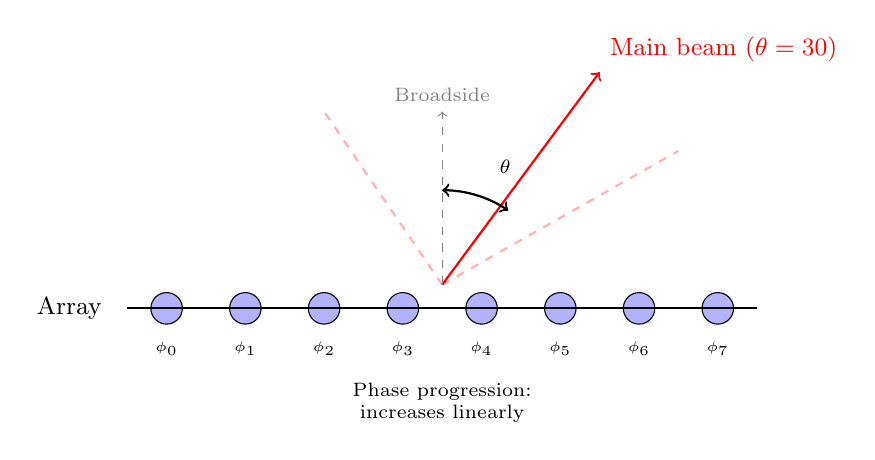
\begin{tikzpicture}[scale=1.0]
% Array elements
\foreach \x in {0,1,2,3,4,5,6,7} {
  \draw[fill=blue!30] (\x,0) circle (0.2);
  \node[below,font=\tiny] at (\x,-0.3) {$\phi_{\x}$};
}

% Array line
\draw[thick] (-0.5,0) -- (7.5,0);
\node[left,font=\small] at (-0.7,0) {Array};

% Beam pattern (simplified)
\draw[red,thick,->] (3.5,0.3) -- (5.5,3) node[above right,font=\small] {Main beam ($\theta = 30°$)};
\draw[red,thick,dashed,opacity=0.3] (3.5,0.3) -- (2,2.5);
\draw[red,thick,dashed,opacity=0.3] (3.5,0.3) -- (6.5,2);

% Broadside reference
\draw[gray,dashed,->] (3.5,0.3) -- (3.5,2.5) node[above,font=\scriptsize,gray] {Broadside};

% Angle annotation
\draw[<->,thick] (3.5,1.5) arc (90:56:1.5);
\node[font=\scriptsize] at (4.3,1.8) {$\theta$};

% Phase progression
\node[font=\scriptsize,align=center] at (3.5,-1.2) {Phase progression:\\increases linearly};

\end{tikzpicture}
\end{center}

\subsection{Array Performance Parameters}

\textbf{Array gain:}
\begin{equation}
G_{\text{array}} = N \cdot G_{\text{element}}
\end{equation}

In decibels:
\begin{equation}
G_{\text{array,dB}} = 10 \log_{10}(N) + G_{\text{element,dB}}
\end{equation}

For 256-element AESA with $G_{\text{element}} = 5$~dBi:
\begin{equation}
G_{\text{array,dB}} = 10 \log_{10}(256) + 5 = 24 + 5 = 29 \text{ dBi}
\end{equation}

\textbf{Beamwidth (half-power):}
\begin{equation}
\theta_{3\text{dB}} \approx \frac{\lambda}{N \cdot d} \quad \text{(radians)}
\end{equation}

For 256 elements with $d = \lambda/2$:
\begin{equation}
\theta_{3\text{dB}} \approx \frac{\lambda}{256 \cdot \lambda/2} = \frac{1}{128} \text{ rad} \approx 0.45°
\end{equation}

\begin{calloutbox}{LPI Advantage}
Narrow beamwidth ($<1°$) concentrates radiated power in a small solid angle, making the signal difficult to intercept from off-axis directions. Combined with low peak power and frequency agility, AESA radars achieve excellent LPI performance.
\end{calloutbox}

\subsection{AESA Applications}

\textbf{APG-77 (F-22 Raptor):}
\begin{itemize}
\item Frequency: X-band (8--12~GHz), 4~GHz agility
\item Array: 2000+ transmit/receive (T/R) modules
\item Power: 13~kW average, 20~kW peak per module
\item Modes: Air-to-air, air-to-ground, SAR, electronic attack
\item Detection range: $>200$~km (fighter-sized target)
\item LPI: Adaptive power, narrow beamwidth (1--2°), low sidelobes ($<-40$~dB)
\end{itemize}

\textbf{AN/SPY-6 (U.S. Navy DDG-51):}
\begin{itemize}
\item Frequency: S-band (3.3--3.5~GHz)
\item Array: 37 Radar Modular Assemblies (RMAs), 5000+ T/R modules
\item Power: 6~MW average radiated power
\item Range: $>300$~km (ballistic missile detection)
\item Capabilities: Track 1000+ targets, adaptive nulling, multi-mission
\end{itemize}

\section{Link 16 (JTIDS)}

Joint Tactical Information Distribution System provides jam-resistant, LPI/LPD tactical data networking.

\subsection{Network Architecture}

\textbf{Participants:}
\begin{itemize}
\item Aircraft: F-15, F-16, F-22, F-35, E-3 AWACS
\item Ships: Aegis cruisers/destroyers, carriers
\item Ground: Patriot SAM, THAAD, command posts
\end{itemize}

\textbf{Topology:} Time Division Multiple Access (TDMA)
\begin{itemize}
\item 128 time slots per 12-second frame
\item Nodes assigned slots (voice/data)
\item Collision-free multiple access
\end{itemize}

\subsection{Link 16 Network Topology}

\begin{center}
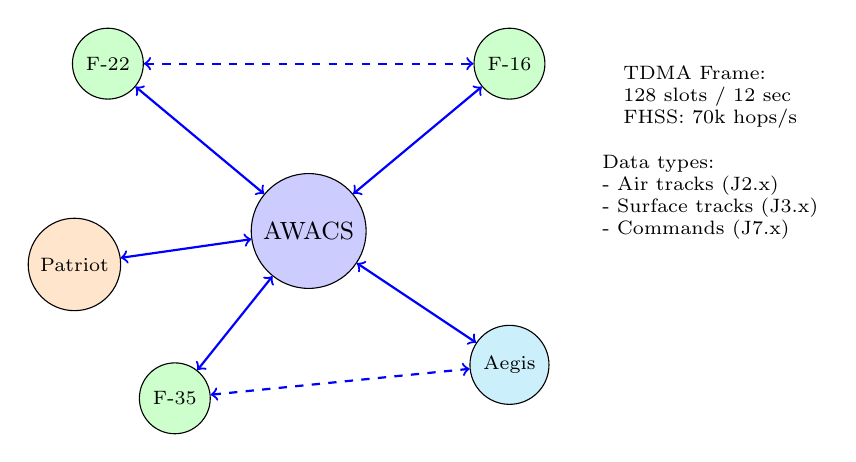
\begin{tikzpicture}[scale=0.85]
% Central node (AWACS)
\node[circle,draw,fill=blue!20,minimum size=1.2cm,font=\small] (awacs) at (0,0) {AWACS};

% Fighter nodes
\node[circle,draw,fill=green!20,minimum size=0.9cm,font=\scriptsize] (f22) at (-3,2.5) {F-22};
\node[circle,draw,fill=green!20,minimum size=0.9cm,font=\scriptsize] (f16) at (3,2.5) {F-16};
\node[circle,draw,fill=green!20,minimum size=0.9cm,font=\scriptsize] (f35) at (-2,-2.5) {F-35};

% Ship node
\node[circle,draw,fill=cyan!20,minimum size=0.9cm,font=\scriptsize] (aegis) at (3,-2) {Aegis};

% Ground node
\node[circle,draw,fill=orange!20,minimum size=0.9cm,font=\scriptsize] (patriot) at (-3.5,-0.5) {Patriot};

% Connections (bidirectional)
\draw[<->,thick,blue] (awacs) -- (f22);
\draw[<->,thick,blue] (awacs) -- (f16);
\draw[<->,thick,blue] (awacs) -- (f35);
\draw[<->,thick,blue] (awacs) -- (aegis);
\draw[<->,thick,blue] (awacs) -- (patriot);
\draw[<->,thick,blue,dashed] (f22) -- (f16);
\draw[<->,thick,blue,dashed] (f35) -- (aegis);

% Legend
\node[align=left,font=\scriptsize] at (6,2) {TDMA Frame:\\128 slots / 12 sec\\FHSS: 70k hops/s};
\node[align=left,font=\scriptsize] at (6,0.5) {Data types:\\- Air tracks (J2.x)\\- Surface tracks (J3.x)\\- Commands (J7.x)};

\end{tikzpicture}
\end{center}

\subsection{Link 16 Waveform Parameters}

\textbf{Physical layer:}
\begin{itemize}
\item Frequency: 960--1215~MHz (L-band)
\item Modulation: MSK (Minimum Shift Keying) -- constant envelope
\item Waveform: FHSS + TDMA hybrid
\item Hop rate: 70,000 hops/second
\item Hop duration: $\sim 14~\mu$s
\item Channels: 51 frequencies (15~MHz spacing)
\item Data rate: 28.8~kbps (typical), up to 115.2~kbps
\end{itemize}

\subsection{Link 16 Processing Gain}

Combined FHSS and TDMA provide multi-layer processing gain:
\begin{equation}
G_{\text{total}} = G_{\text{FH}} + G_{\text{TDMA}}
\end{equation}

Frequency hopping gain:
\begin{equation}
G_{\text{FH,dB}} = 10 \log_{10}(51) = 17 \text{ dB}
\end{equation}

Time diversity gain:
\begin{equation}
G_{\text{TDMA,dB}} = 10 \log_{10}(128) = 21 \text{ dB}
\end{equation}

Total processing gain:
\begin{equation}
G_{\text{total}} = 17 + 21 = 38 \text{ dB}
\end{equation}

\subsection{TRANSEC and Synchronization}

\textbf{Cryptographic hopping pattern generation:}
\begin{itemize}
\item Input: Network ID + GPS time + Crypto key (KY-58/KG-84)
\item Output: Pseudorandom frequency sequence
\item Pattern period: Classified (days to months, appears never-repeating)
\item Synchronization: GPS time $\pm 100~\mu$s accuracy required
\item Anti-spoofing: Time-of-Transmission (TOT) authentication
\end{itemize}

\section{Worked Example: Link 16 Jamming Margin}

\textbf{Problem:} Calculate the jamming margin for a Link 16 tactical data link under enemy jamming.

\textbf{Given:}
\begin{itemize}
\item Processing gain: $G = 38$~dB (FHSS + TDMA)
\item Jammer-to-signal ratio: $J/S = 50$~dB (jammer 100~km away)
\item Required $E_b/N_0 = 12$~dB (MSK with FEC)
\item Implementation losses: $L = 3$~dB
\end{itemize}

\textbf{Required:} Determine if link survives and identify countermeasures.

\textbf{Solution:}

\textit{Step 1: Calculate initial jamming margin.}

Using Equation~(4):
\begin{equation}
M_{\text{jam}} = G - J/S - (E_b/N_0)_{\text{req}} - L
\end{equation}
\begin{equation}
M_{\text{jam}} = 38 - 50 - 12 - 3 = -27 \text{ dB}
\end{equation}

\textbf{Result:} $M_{\text{jam}} < 0$ --- LINK FAILS.

\textit{Step 2: Apply directional antenna countermeasure.}
\begin{itemize}
\item Antenna gain toward participant: $+10$~dBi
\item Null depth toward jammer: $-20$~dB
\item Front-to-back ratio: 30~dB
\end{itemize}

Effective jammer-to-signal ratio:
\begin{equation}
J/S_{\text{effective}} = 50 - 30 = 20 \text{ dB}
\end{equation}

Revised jamming margin:
\begin{equation}
M_{\text{jam}} = 38 - 20 - 12 - 3 = 3 \text{ dB}
\end{equation}

\textbf{Answer:} With directional antenna, $M_{\text{jam}} = +3$~dB --- LINK SURVIVES.

\textbf{Interpretation:} The 3~dB margin provides minimal protection. For robust operation, additional countermeasures such as adaptive power control or higher-gain antennas would be recommended to achieve $M_{\text{jam}} \geq 10$~dB.

\section{Covert Communications}

\subsection{Objective}

Transmit data undetected by adversary signals intelligence (SIGINT) systems through Low Probability of Detection (LPD) techniques.

\subsection{Ultra-Wideband Spread Spectrum}

For covert communications, ultra-wideband (UWB) spread spectrum achieves LPD by spreading the signal power so thinly that it appears as thermal noise.

\textbf{Example parameters:}
\begin{itemize}
\item Data rate: $R_b = 1$~kbps
\item Spread bandwidth: $BW = 1$~GHz
\item Transmit power: $P_{TX} = 1$~W
\end{itemize}

Processing gain:
\begin{equation}
G = \frac{BW}{R_b} = \frac{10^9}{10^3} = 10^6 \quad (60 \text{ dB})
\end{equation}

Transmitted power spectral density:
\begin{equation}
\text{PSD} = \frac{P_{TX}}{BW} = \frac{1 \text{ W}}{10^9 \text{ Hz}} = 10^{-9} \text{ W/Hz} = -90 \text{ dBm/Hz}
\end{equation}

Per MHz:
\begin{equation}
\text{PSD}_{\text{MHz}} = -90 + 10 \log_{10}(10^6) = -30 \text{ dBm/MHz}
\end{equation}

Thermal noise floor (per MHz):
\begin{equation}
N_{\text{MHz}} = -174 \text{ dBm/Hz} + 10 \log_{10}(10^6) = -114 \text{ dBm/MHz}
\end{equation}

\begin{keyconcept}
The signal PSD ($-90$~dBm/Hz) is 24~dB below the thermal noise floor ($-114$~dBm/MHz when integrated over 1~MHz). Even sensitive intercept receivers cannot distinguish the transmission from background noise without knowledge of the spreading code and precise synchronization.
\end{keyconcept}

\subsection{Spread Spectrum Below Noise Floor Visualization}

\begin{center}
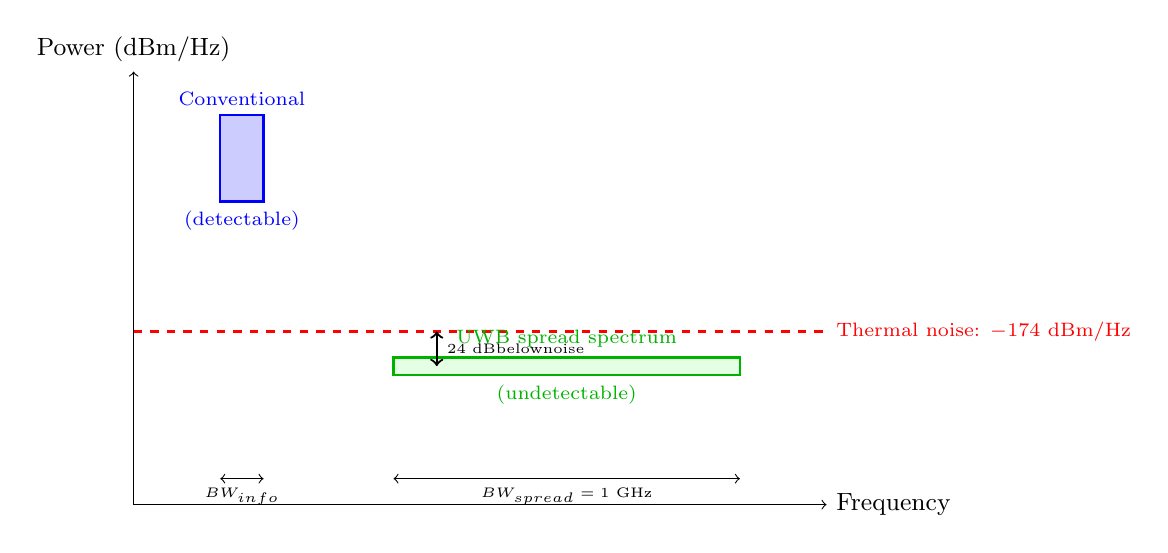
\begin{tikzpicture}[scale=1.1]
% Axes
\draw[->] (0,0) -- (8,0) node[right,font=\small] {Frequency};
\draw[->] (0,0) -- (0,5) node[above,font=\small] {Power (dBm/Hz)};

% Noise floor
\draw[thick,red,dashed] (0,2) -- (8,2);
\node[right,font=\scriptsize,red] at (8,2) {Thermal noise: $-174$ dBm/Hz};

% Narrowband signal (conventional)
\draw[thick,blue,fill=blue!20] (1,4.5) rectangle (1.5,3.5);
\node[above,font=\scriptsize,blue] at (1.25,4.5) {Conventional};
\node[below,font=\scriptsize,blue] at (1.25,3.5) {(detectable)};

% Spread spectrum signal (below noise)
\draw[thick,green!70!black,fill=green!10] (3,1.5) rectangle (7,1.7);
\node[above,font=\scriptsize,green!70!black] at (5,1.7) {UWB spread spectrum};
\node[below,font=\scriptsize,green!70!black] at (5,1.5) {(undetectable)};

% Annotations
\draw[<->,thick] (3.5,1.6) -- (3.5,2) node[midway,right,font=\tiny] {24 dB\\below\\noise};

% Bandwidth indicators
\draw[<->,thin] (1,0.3) -- (1.5,0.3) node[midway,below,font=\tiny] {$BW_{\text{info}}$};
\draw[<->,thin] (3,0.3) -- (7,0.3) node[midway,below,font=\tiny] {$BW_{\text{spread}} = 1$ GHz};

\end{tikzpicture}
\end{center}

\subsection{Additional Covert Techniques}

\textbf{Steganography in OFDM:}
\begin{itemize}
\item Hide data in unused subcarriers or modulate pilot tone phases
\item OFDM pilot modulation: Covert channel up to 1~Mbps (802.11a)
\item Null subcarrier insertion: Low-power data on reserved frequencies
\item Detection challenge: Requires statistical analysis or wideband monitoring
\end{itemize}

\textbf{Time-domain hiding:}
\begin{itemize}
\item Insert ultra-short bursts in inter-frame gaps (e.g., WiFi SIFS)
\item Covert capacity: $\sim 6$~Mbps using 6.25\% duty cycle
\item Detection: Appears as multipath or transient interference
\end{itemize}

\section{Applications}

\subsection{GPS M-Code}

\textbf{Systems:} JDAM precision bombs, Tomahawk cruise missiles, Excalibur artillery, fighter avionics (F-22, F-35, B-2)

\textbf{Performance:}
\begin{itemize}
\item Positioning accuracy: $<1$~m horizontal, $<3$~m vertical
\item Time accuracy: $<10$~ns (critical for network synchronization)
\item Anti-jam: Survives 60+ dB jamming with CRPA
\end{itemize}

\subsection{MILSTAR/MUOS Satellites}

\textbf{Systems:} Strategic and tactical military satellite communications

\textbf{Capabilities:}
\begin{itemize}
\item Data rates: 75~bps to 1.544~Mbps (T1)
\item Coverage: Global (5 GEO satellites)
\item Jam resistance: 30~dB processing gain + directional antennas
\item Security: NSA Type 1 encryption
\end{itemize}

\subsection{Link 16 (JTIDS)}

\textbf{Platforms:} F-15, F-16, F-22, F-35, E-3 AWACS, Aegis ships, Patriot SAM, THAAD

\textbf{Function:} Real-time tactical data exchange (air tracks, surface tracks, commands)

\textbf{Performance:}
\begin{itemize}
\item Update rate: 5--10~seconds (air tracks), 30--60~seconds (surface)
\item Jam resistance: 38~dB processing gain (FHSS + TDMA)
\item Range: Line-of-sight (300+ km air-to-air)
\end{itemize}

\subsection{AESA Radars}

\textbf{Systems:}
\begin{itemize}
\item APG-77 (F-22 Raptor): 2000+ T/R modules, >200~km detection range
\item AN/SPY-6 (Navy DDG-51): 5000+ T/R modules, track 1000+ targets
\item AN/TPY-2 (THAAD): 25,344 elements, 1000+~km missile detection
\end{itemize}

\textbf{Capabilities:} LPI operation, electronic attack, multi-mission (air defense, ballistic missile defense, surface search)

\section{Summary}

\subsection{Performance Comparison}

\begin{center}
\begin{tabular}{lcccc}
\toprule
\textbf{Technique} & \textbf{Processing Gain} & \textbf{Primary Benefit} & \textbf{Applications} \\
\midrule
DSSS & 20--40 dB & AJ, LPI & GPS M-code, tactical radios \\
FHSS & 17--30 dB & LPD, follower-jam resist & MILSTAR, Link 16 \\
AESA & N/A (spatial) & LPI, multi-target & APG-77, AN/SPY-6 \\
Nulling Antenna & 20--40 dB & Jammer rejection & CRPA, adaptive arrays \\
FEC & 3--10 dB & Error correction & All systems \\
Encryption & N/A & Content security & All military systems \\
\bottomrule
\end{tabular}
\end{center}

\subsection{Key Performance Metrics}

\begin{center}
\begin{tabular}{ll}
\toprule
\textbf{Parameter} & \textbf{Typical Value} \\
\midrule
Processing gain (DSSS) & 20--50 dB \\
Processing gain (FHSS) & 17--30 dB \\
Jamming margin (required) & $\geq 10$ dB \\
LPD threshold & Signal PSD $<$ Noise floor \\
CRPA null depth & 30--40 dB \\
GPS M-code accuracy & $<1$ m horizontal \\
Link 16 update rate & 5--10 seconds \\
AESA beamwidth & $<1°$ (narrow) \\
\bottomrule
\end{tabular}
\end{center}

\textbf{Advantages:}
\begin{itemize}
\item Jam resistance: Links survive jammers 1000--10,000$\times$ stronger
\item LPI/LPD: Signals operate below noise floor, undetectable to wideband receivers
\item Security: Multiple layers (spread spectrum, encryption, authentication)
\item Flexibility: Adaptive coding, power management, multi-mission capability
\item Reliability: Proven in GPS, SATCOM, tactical data links, radar systems
\end{itemize}

\textbf{Disadvantages:}
\begin{itemize}
\item Complexity: Requires sophisticated signal processing, synchronization
\item Cost: AESA radars and SAASM receivers are expensive
\item Bandwidth: Spread spectrum occupies wide frequency ranges
\item Latency: TDMA and hopping introduce timing delays
\item Power: Some techniques (AESA) require high transmit power
\end{itemize}

\textbf{Best suited for:} Military and government applications requiring anti-jam capability, covert operation, and secure communications in hostile electromagnetic environments.

\section{Further Reading}

\subsection{Related Chapters}

\begin{itemize}
\item Chapter~\ref{ch:spread-spectrum}: Spread Spectrum (DSSS/FHSS) -- Technical foundation for AJ/LPI
\item Chapter~\ref{ch:snr}: Signal-to-Noise Ratio (SNR) -- Link budget fundamentals
\item Chapter~\ref{ch:ber}: Bit Error Rate (BER) -- Performance analysis
\item Chapter~\ref{ch:awgn}: Additive White Gaussian Noise (AWGN) -- Channel modeling
\item Chapter~\ref{ch:fec}: Forward Error Correction (FEC) -- Coding gain
\end{itemize}

\subsection{Textbooks}

\begin{itemize}
\item \textbf{Poisel}, \emph{Introduction to Communication Electronic Warfare Systems} -- Comprehensive EW treatment
\item \textbf{Torrieri}, \emph{Principles of Spread-Spectrum Communication Systems} (4th ed.) -- Modern military focus
\item \textbf{Skolnik}, \emph{Radar Handbook} (3rd ed.) -- Phased arrays, AESA, LPI radar
\item \textbf{Adamy}, \emph{EW 101: A First Course in Electronic Warfare} -- Accessible intro to jamming/AJ
\end{itemize}

\subsection{Military Standards}

\begin{itemize}
\item \textbf{MIL-STD-188-181}: US DoD FHSS standard
\item \textbf{GPS ICD-IS-800}: M-code interface control document (FOUO)
\item \textbf{Link 16 MIDS JTIDS STD}: Message standards (NATO STANAG 5516)
\end{itemize}
